\documentclass[11pt,a4]{article}
\usepackage[pdftex]{graphicx}
\begin{document}
\section{LightSensor}
There are many sensors that may be used to determine the transparancy and/or colour of an object, yet within the standard sensor selection of LEGO Mindstorm\textregistered  the LightSensor is an abvious choice. Choosing a standard component generally has the following advantags and disadvantages.
\noindent Advantages
\begin{itemize}
    \item Readily available.
    \item Tried and proven.
    \item Support and API already implemented.
    \item Cheap in low numbers
\end{itemize}
\noindent Disadvantages
\begin{itemize}
    \item General purpose, meaning designed for more that just for transparancy and colour detection. This means that the LightSensor may not be as efficient or accurate as if it was specifically designed for the purpose.
    \item Expensive in high numbers.
\end{itemize}
For this assignment the standard LightSensor should be sufficient, yet to be sure a series of tests and analysis should be performed.
\subsection{Characteristics}
The LEGO LightSensor can operated in two modes; ambient and reflective. Ambient means that it measures the light level using simple passive measurements. This form of sensor is often used to detect the LUX-count in a room, indicating the rooms adequacy for office space with respect to light. The reflective mode is an active mode, where a flood-light (red LED) is activated and the reflected light is measured.

It would be possible to use the ambient mode to detect transparancy, if a stationary light-source was placed across form the sensor and the items to measure be transported between the light source and the sensor.

An alternative is to use the reflective mode to register how much light is reflected of the item, thereby measuring transparancy.

Both solutions will be sensitive to changes in the surrounding light-level, as normal light ("white" light), is a broad spectrum light containing elements of all colours, so there is no way to filter out specific frequencies, even if the sensor allowed such filtering, which it does not. 

There are alternative ways to solve this. Minimizing changes in surrounding light-level is obviously a good solution. This may be done by shielding the sensor and item being measured (using a fixed, stationary light source inside the shielding to generate some light may be needed, and is mandetory in the ambient mode). This may be augmented by continous calibration of the sensor, thereby filtering out slow changes in the surrounding light-level. A final solution is to simply place the entire setup in a room with a fixed stationary light-source and with no uncontrollable light-sources or shadow-casters (e.g. windows and people). What level of shielding and continous calibration is required should be the subject of further analysis.

The way the LightSensor "sees" in reflective mode is by detecting how much light is reflected by the object in front of the sensor. The flood-light source is a red LED operating in the infrared spectrum, just under visible light, yet unfortunately the sensor is not able to only operate in this spectrum, and the entire spectrum is detected by the sensor. Had the sensor been configurable to only receive the infra-red reflections it would not have been a total solution, as normal "white" light contains all frequencies, incl. infra-red. In order for the sensor to eliminate external light-sources the sensor must be calibrated, thereby allowing it to ignore the general light in the room, as long as that light does not change. What the sensor "sees" is an integer which, in normalized form, range from 0 to 1023. This value may be translated to a form of gray-scale representation of the "colour" of the item in front of the sensor. Unfortunately this does not match well with transparency, as a transparent object will be indistinguishable from a black object, as neither will reflect any light (ideally transparent and ideally black). Placing an external lightsource across from the sensor may solve this problem, or perhaps the assignement should be altered to sort by colour not transparency??? The accuracy of the LightSensor at different distances from the object, and in different external light levels should be the subject of further analysis.

Knowing that the external light sources may change also means that faulty readings may occur until a new callibration can be performed. An importent step to avoiding faulty behaviour is to detect these readings as faulty before any action is taken. One way of filtering out bad reading is to take multiple reading before making a decision, which allows for a single faulty reading being detected and ignored. For this to be possible the sampling and detection of the LightSensor must be considerably faster than the movement of the conveyor belt. Asuming the conveyor belt is moving a 1m/s and the object is 5cm long, and we wish to have 10 samples within the object, we muct perform samling at 200Hz, as 5cm is covered in 50ms and 10 samples in 20ms requries one sample per 2ms, or 200Hz. The equation is Hz = (<conveyor speed>[m/s] / <object size>[m]) * <sample count>. It may be possible to sample at 200Hz, but this does not mean that the sensor is able to function at this speed. It depends on its reactivity - how long it tages a change in the external condition to manifest in the analog reading. If the sensor is sluggish, meaning that a light-change has to be present for e.g. 10ms before the analog value is updated, it will not be possible to operate the sensor at 200Hz. The reaction time of the light sensor along with the possible samling speed must be the subject of further analysis.

We may also need to recalibrate when the light in the room changes. This could be done by determining that the sensor is between items and then comparing the reading to the calibration value. If it differs it is time for a recalibration. Whether such an on-the-fly calibration is possible must be the subject of further analysis.

\noindent Analysis required
\begin{itemize}
    \item Reactiontime of LightSensor.
    \item Accuracy of LightSensor as function of distance to object
    \item Accuracy of LightSensor as function of external light source
    \item LightSensor sensitivity to external light changes.
    \item LightSensor sampling frequency range and main processor operating frequency
    \item LightSensor calibration performance.
\end{itemize}

\subsection{Analysis}
The analysis consists of writing a set of small test programs and creating some test-setups to shed some light (no pun intended) on the LightSensor, with respect to the issues mentioned above. 

In Figure ~\ref{fig:lightsensor_analysis} and Table may be seen a hyphothetical test-setup, including "all" the parameters of interest. 

\begin{figure}[jpg]
\centering
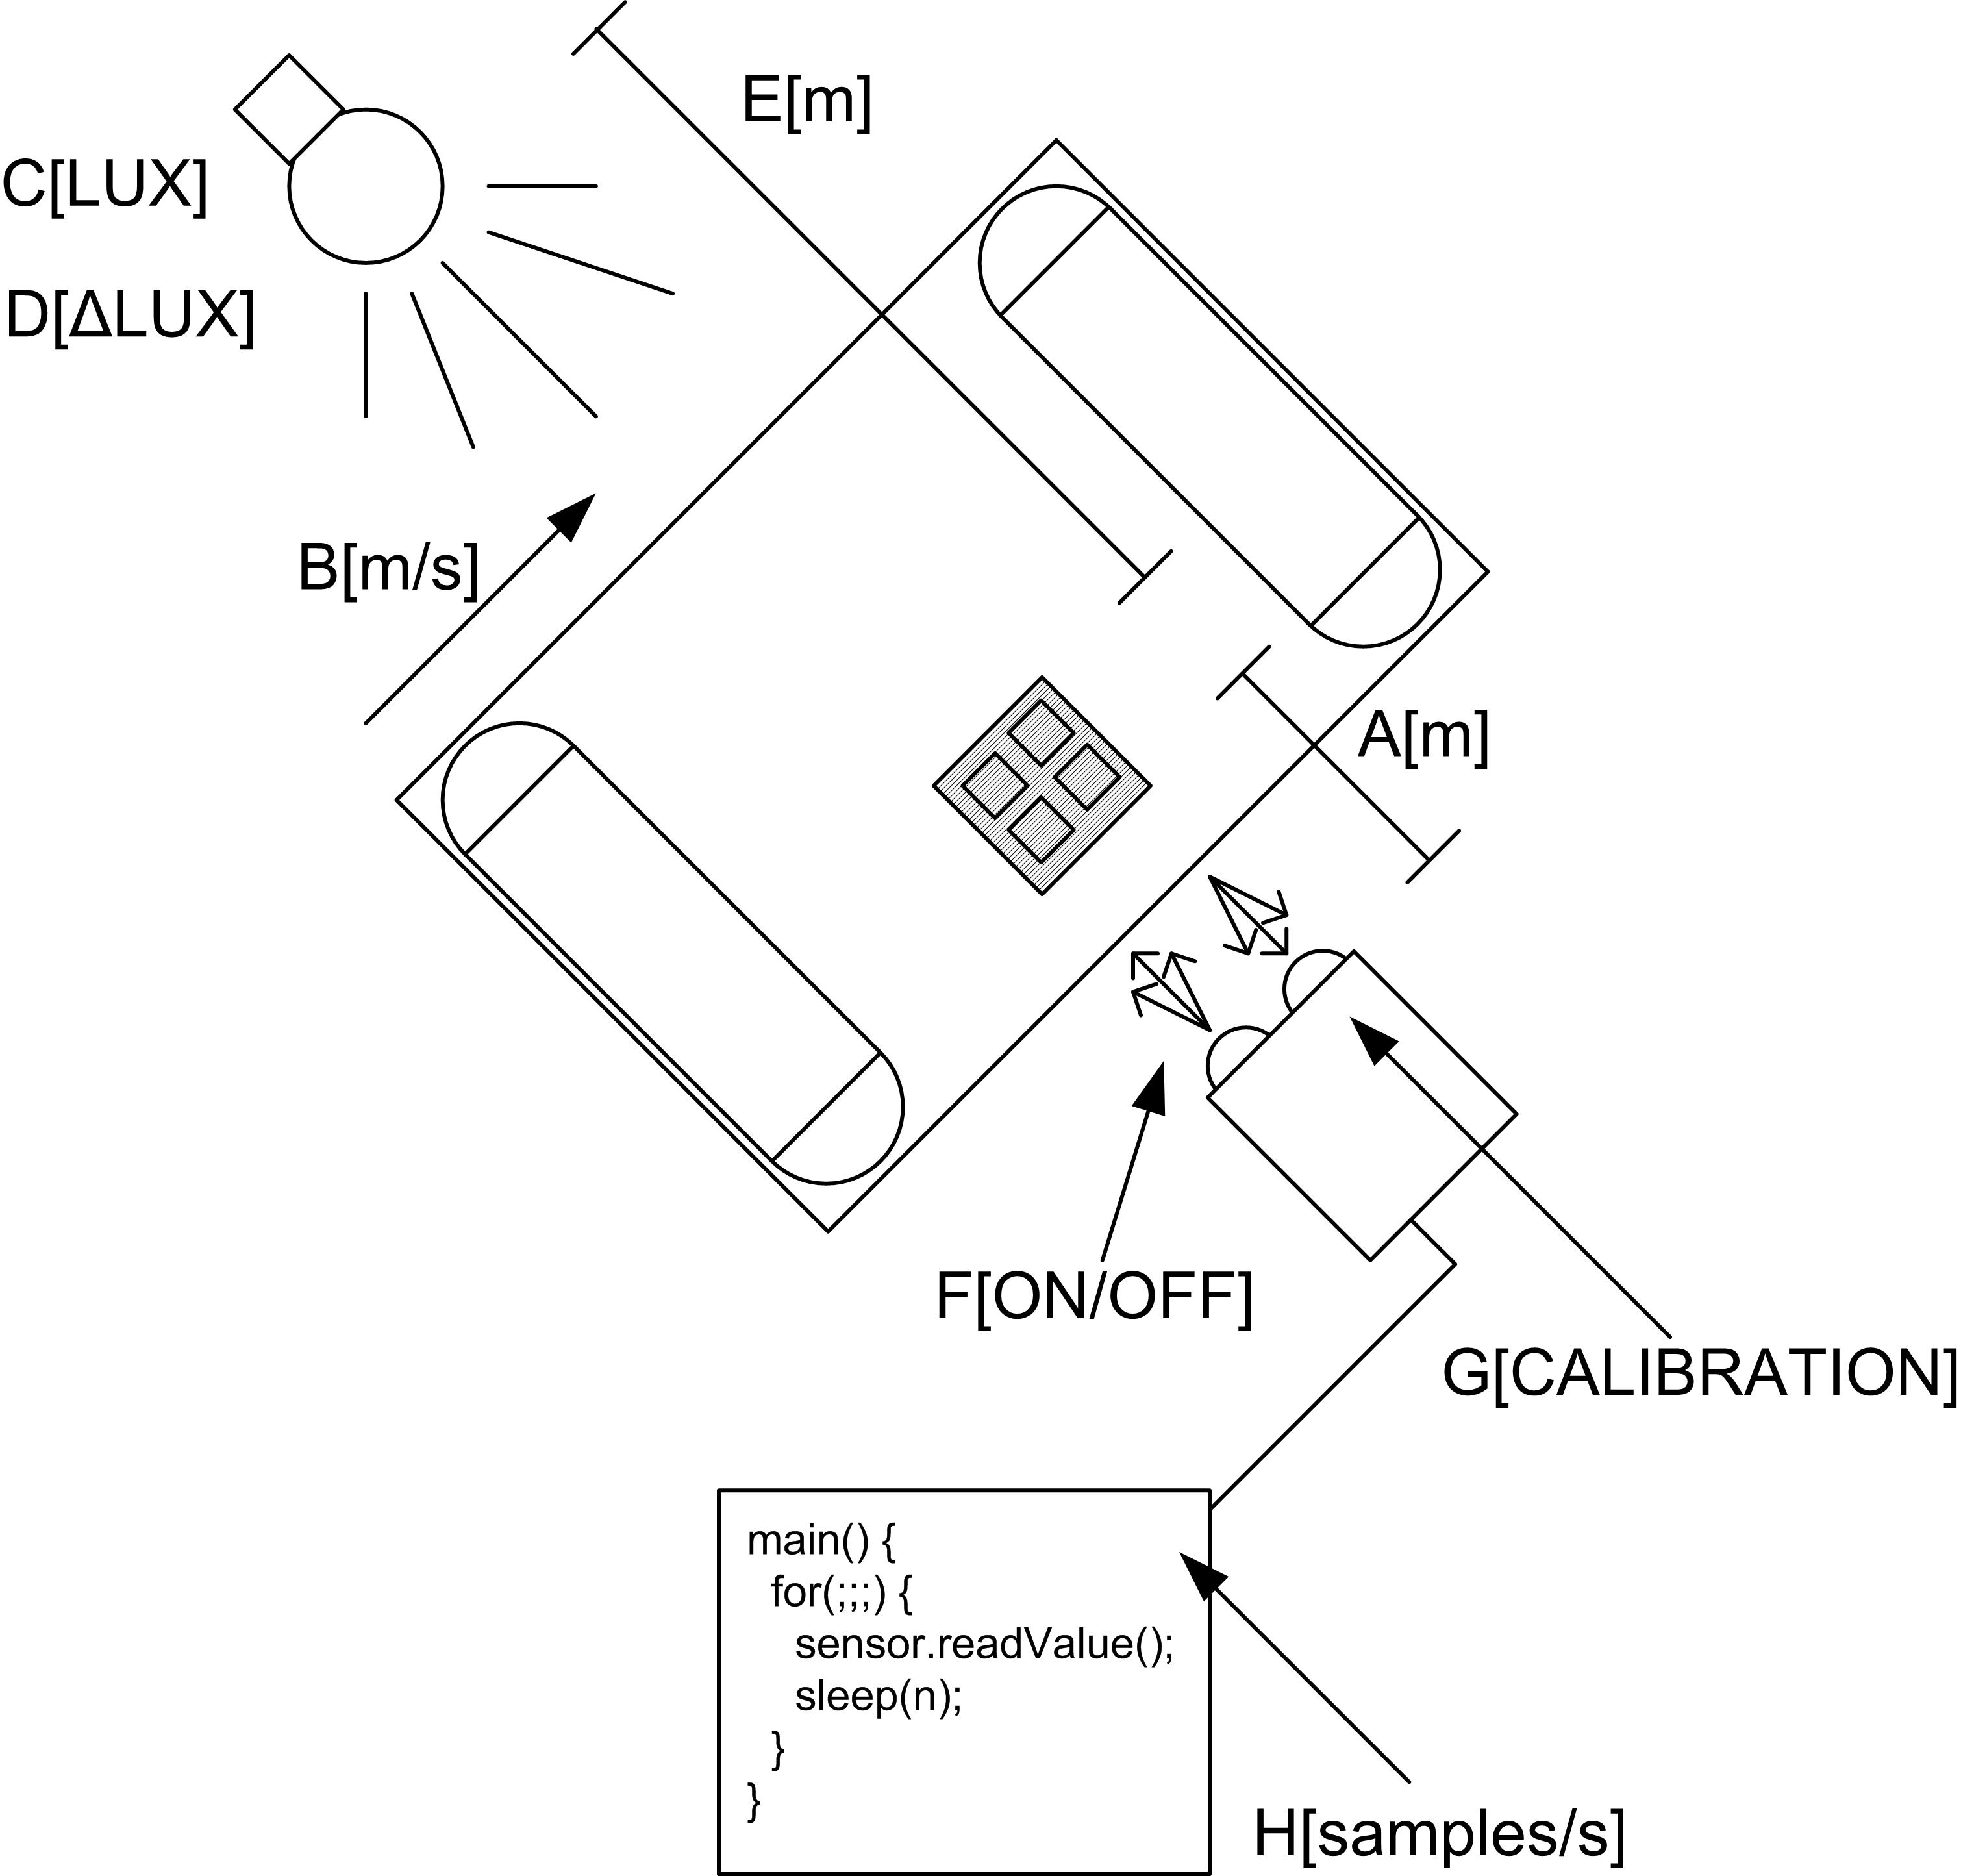
\includegraphics{lightsensor_analysis}
\caption{LightSensor analysis setup}
\label{fig:lightsensor_analysis_setup}
\end{figure}

\begin{table}[ht]
\caption{LightSensor analysis setup description}
\centering
\begin{tabular}{c c}
\hline\hline
ID & Description \\ [0.5ex]
\hline
A & The distance from the LightSensor to the object it is sensing. \\* This is important to measure in order to determine the optimal \\* location of the LightSensor relative to the objects on the conveyer-belt, \\* so as to achieve the most accurate readings. This may be tested by moving \\* the LightSensor relative to the object and logging the reading-accuracy \\
B & The speed of the conveyer-belt. This is very important, \\* as the sampling frequency and the response-time of the LightSensor is directly\\* related to the maximum speed of the conveyer-belt. To determine the response-time,\\* a simple program samling at maximum speed may be written,\\* and the speed of the conveyer-belt increased until sampling fails \\* (either due to sampling frequency insufficient or response-time issues) \\
C & The light in the room may have profound effect on the \\* LightSensors accuracy, and this may be tested by running identical tests, \\* but with different external light levels. (no sampling should be done \\* during the level change). \\
D & The change in lighting may also affect the accuracy of the \\* readings. This can be determined by sampling while the lighting is being \\* turned up or down. \\
E & The location of the external light source relative to the \\* object being sensed and the LightSensor is also important. This may be \\* measured by moving the light source while sampling. \\
F & Whether the flood-light of the LightSensor is on may \\* affect the accuracy of the readings \\
G & The calibration of the LightSensor will affect the \\* readings, and testing for the best configuration is very important, as well \\* as determining configuration drift during operation and the possibility \\* of re-calibrating. \\
H & The sampling frequency is also important, as it may \\* be that the response-time of the sensor is faster than the max sample-rate, \\* making the sample-rate the important configuration or vice versa. It \\* should be determined what sampling frequency can be achieved, also under \\* the condition of servicing other peripherals. \\ [1ex]
\hline
\end{tabular}
\label{table:lightsensor_analysis_setup_description}
\end{table}
As the test programs are relatively simple, the builk of the work is in the test-setup. As most of the 
Moving C, D, E together
\end{document}

